\documentclass[11pt,a4paper]{article}

% ML/AI research packages
\usepackage[margin=1in]{geometry}
\usepackage{graphicx}
\usepackage{amsmath}
\usepackage{amsfonts}
\usepackage{amssymb}
\usepackage{booktabs}
\usepackage[hyphens]{url}
\usepackage[hidelinks]{hyperref}
\usepackage{caption}
\usepackage{subcaption}
\usepackage{siunitx}
\usepackage{float}
\usepackage{authblk}

% Title structure
\title{\Large\bfseries Muon Optimizer Hyperparameter Optimization:\\[0.3em]
\large A Systematic Ablation Study for Language Model Training}

% Author structure
\author[1]{Vuk Rosić}
\author[2]{Claude}
\author[3]{Gemini}
\affil[1]{Óbuda University, \texttt{vukrosic1@gmail.com}}
\affil[2]{Anthropic}
\affil[3]{Google}

\date{\today}

\begin{document}
\maketitle

% Code/data links
\begin{center}
\textbf{\href{https://github.com/vukrosic/muon-optimizer-study}{GitHub Repository}}
\end{center}

% Abstract with performance numbers
\begin{abstract}
This paper presents a comprehensive ablation study on the Muon optimizer, investigating optimal hyperparameter configurations for language modeling tasks. We systematically evaluate 18 distinct configurations across three critical dimensions: learning rate (\{0.0312, 0.0625, 0.1250\}), momentum (\{0.8750, 0.9375\}), and Newton-Schulz iteration steps (\{4, 8, 16\}). Training was conducted on the HuggingFaceTB/smollm-corpus using a MinimalLLM architecture (128d, 2L, 4H) for 1500 steps with batch size 32. Our findings reveal that lower learning rates significantly improve performance, with the optimal configuration (LR: 0.0312, Momentum: 0.8750, 4 Steps) achieving a validation loss of 4.3998 compared to the worst-performing variant at 5.9199. The study demonstrates a clear performance hierarchy: configurations with LR 0.0312 consistently outperform higher learning rates by 8.9-34.5\%. Training efficiency varies minimally across Newton-Schulz steps (130-159 seconds), while momentum settings show nuanced effects on convergence stability. These results provide empirical guidance for practitioners implementing Muon optimization in resource-constrained language modeling scenarios.
\end{abstract}

% Key visuals
\begin{figure}[H]
    \centering
    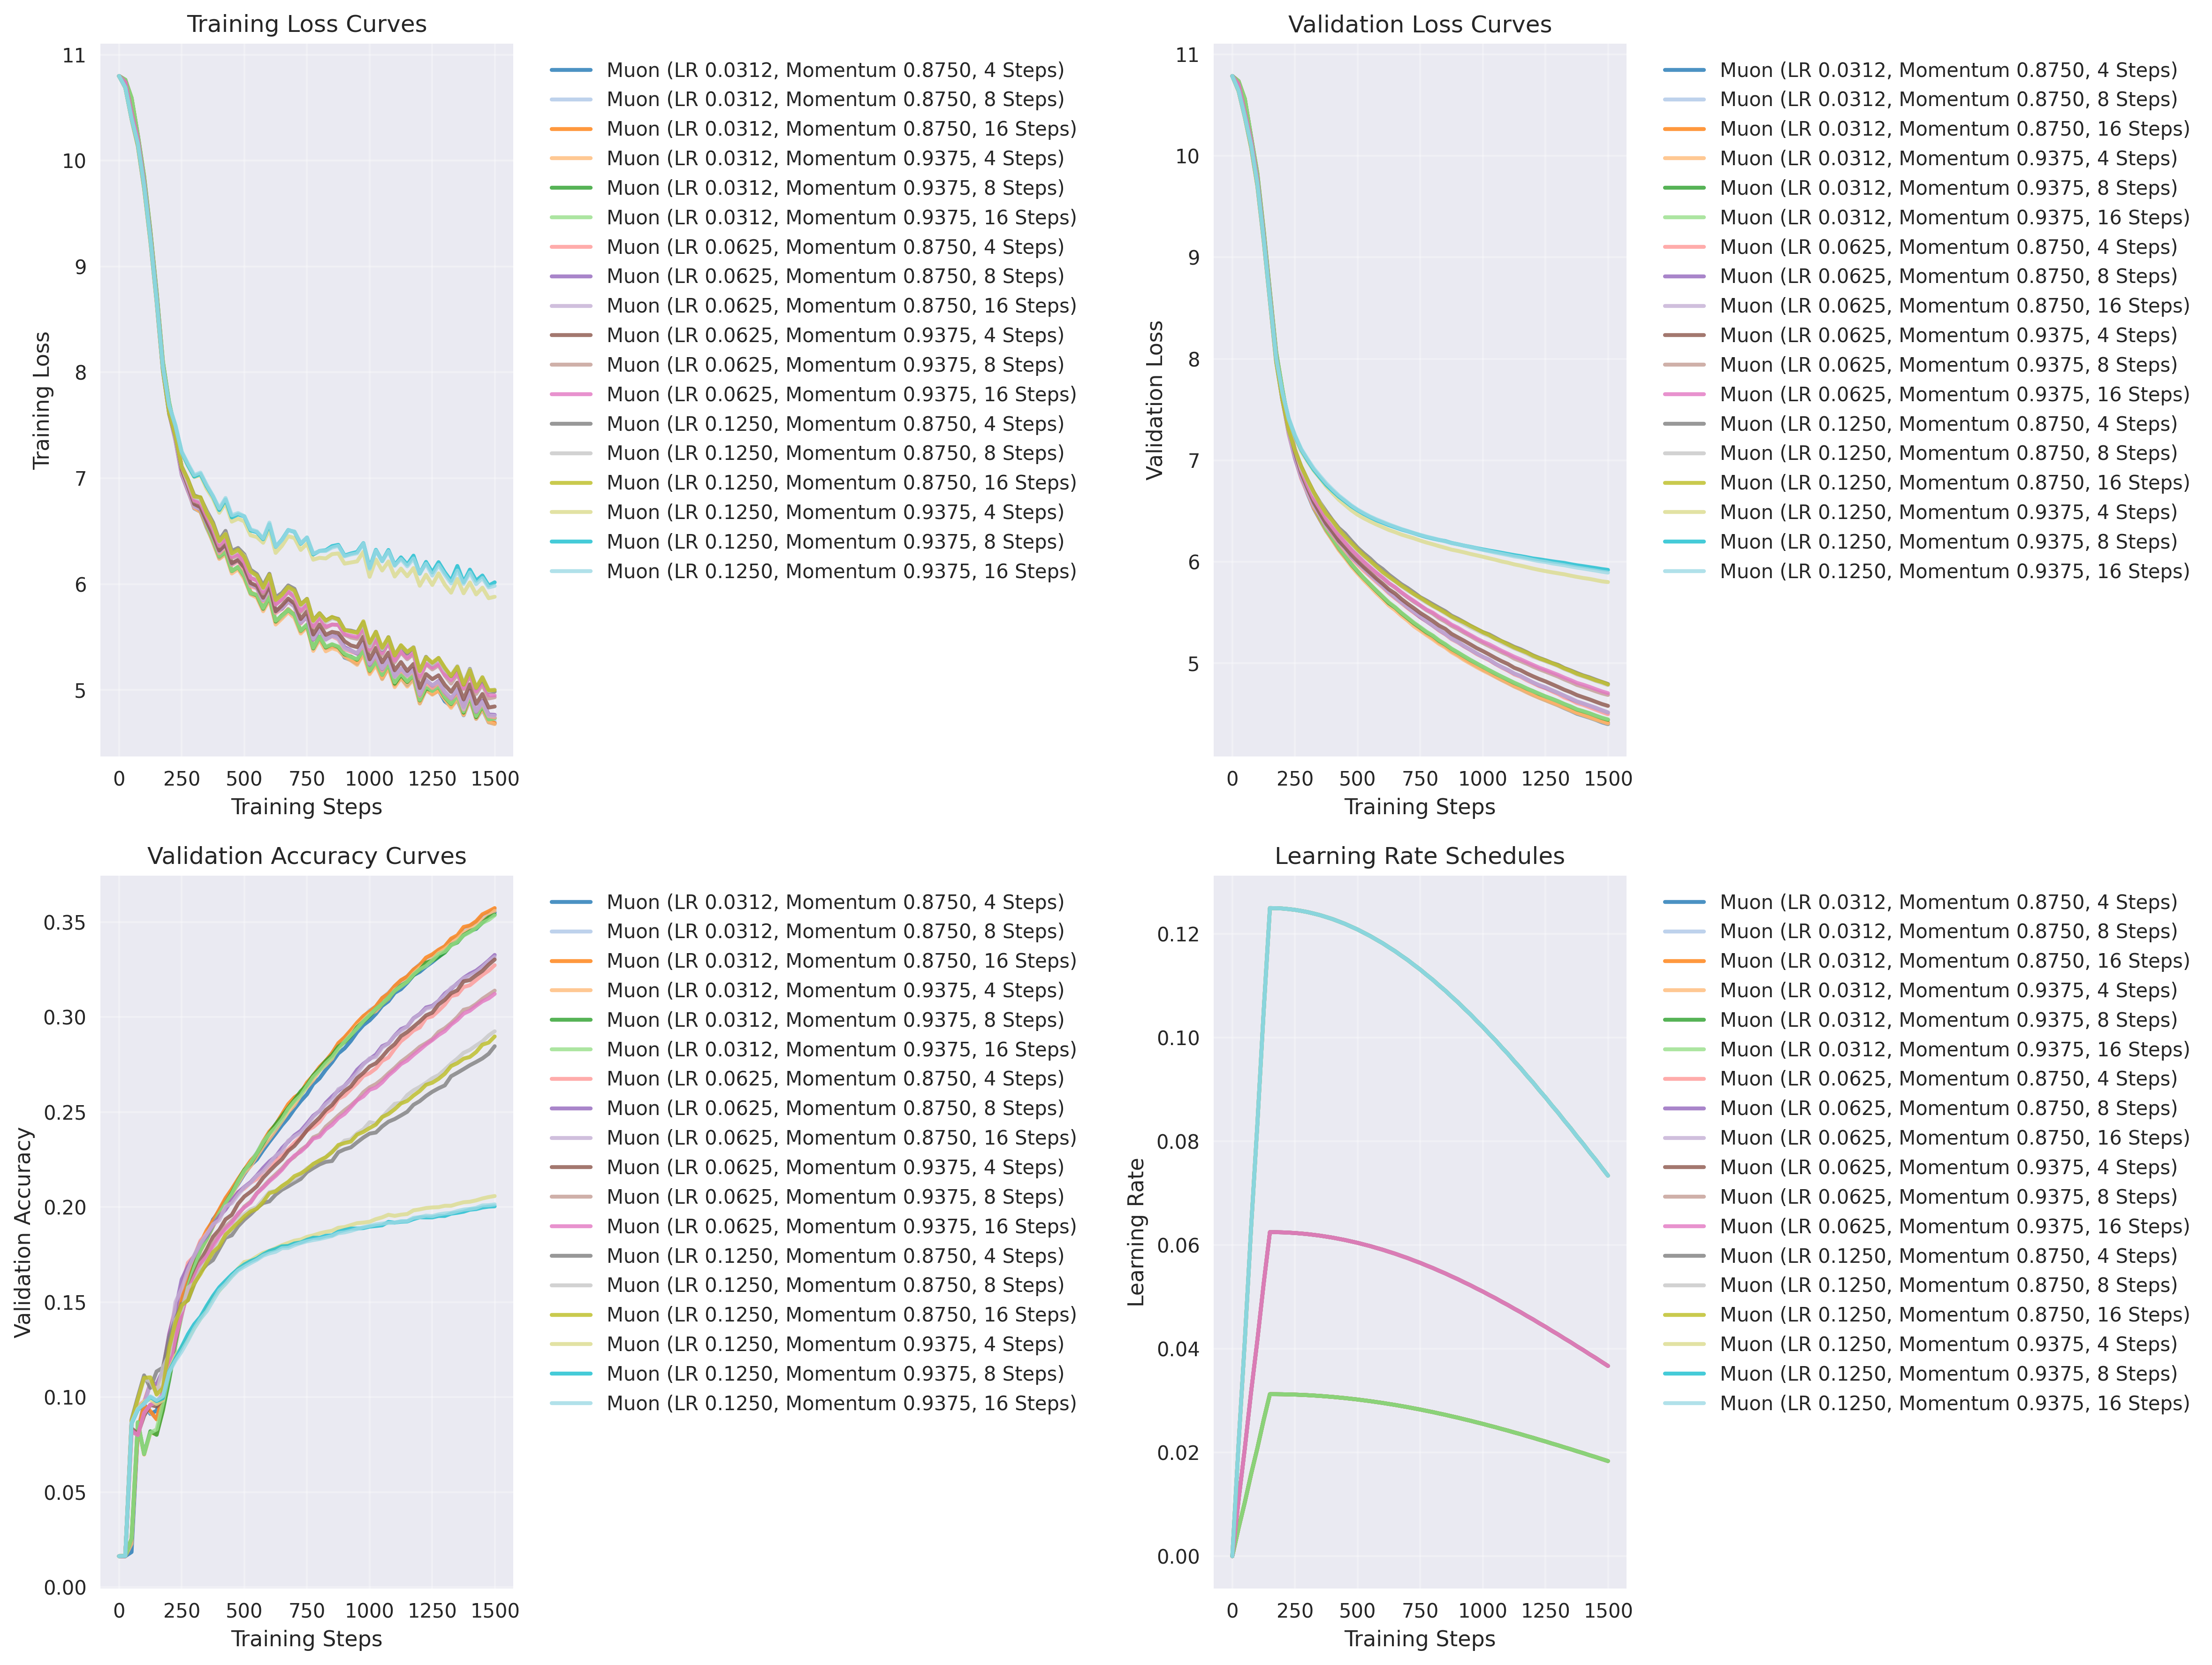
\includegraphics[width=\textwidth]{images/training_curves.png}
    \caption{Training dynamics showing loss convergence, validation accuracy progression, and learning rate schedules across all configurations.}
\end{figure}


\section{Introduction}

Optimizer selection and hyperparameter tuning represent critical factors in deep learning model performance, particularly for language modeling tasks where computational resources are often constrained. The Muon optimizer, incorporating Newton-Schulz iterations for gradient transformation, presents a novel approach to optimization that requires systematic investigation to understand its optimal configuration space.

This paper presents a systematic study examining how three key hyperparameters affect Muon optimizer performance in language modeling: learning rate scaling, momentum coefficients, and Newton-Schulz iteration counts. We investigate 18 distinct configurations across multiple performance dimensions:

\begin{enumerate}
    \item \textbf{Learning Rate Sensitivity:} Three logarithmically-spaced learning rates (0.0312, 0.0625, 0.1250)
    \item \textbf{Momentum Dynamics:} Two momentum values (0.8750, 0.9375) representing different gradient accumulation strategies
    \item \textbf{Newton-Schulz Iterations:} Step counts (4, 8, 16) affecting gradient transformation precision
    \item \textbf{Computational Efficiency:} Training time and convergence characteristics across configurations
\end{enumerate}

Our experiments provide empirical insights for practitioners working with transformer architectures under computational constraints, specifically addressing the trade-offs between optimization effectiveness and training efficiency in small-scale language models.

\section{Methodology}

\subsection{Model Architecture}
We employ a MinimalLLM architecture designed for efficient experimentation while maintaining representativeness of larger language models:

\begin{itemize}
    \item \textbf{Model Dimension (d\_model):} 128 for compact representation learning
    \item \textbf{Layers (n\_layers):} 2 transformer blocks for reduced computational overhead
    \item \textbf{Attention Heads (n\_heads):} 4 multi-head attention mechanisms
    \item \textbf{Feed-Forward Dimension (d\_ff):} 512 (4× model dimension following standard scaling)
    \item \textbf{Vocabulary Size:} Standard tokenizer vocabulary for text processing
    \item \textbf{Sequence Length:} 256 tokens per training sequence
\end{itemize}

\subsection{Dataset and Training Configuration}
\begin{itemize}
    \item \textbf{Dataset:} HuggingFaceTB/smollm-corpus (cosmopedia-v2 split) with 1000 documents
    \item \textbf{Tokenization:} Approximately 200,000 tokens total training data
    \item \textbf{Training Steps:} 1500 steps for comprehensive convergence analysis
    \item \textbf{Batch Size:} 32 samples per gradient update
    \item \textbf{Evaluation Frequency:} Metrics recorded every 25 training steps
    \item \textbf{Base Learning Rate:} 0.01 (scaled by experimental factors)
    \item \textbf{Hardware:} Standard GPU training environment
\end{itemize}

\subsection{Experimental Design}
We performed a systematic grid search over Muon optimizer hyperparameters:

\begin{table}[H]
\centering
\caption{Muon Optimizer Hyperparameter Grid}
\label{tab:hyperparameter_grid}
\begin{tabular}{@{}lcc@{}}
\toprule
\textbf{Hyperparameter} & \textbf{Values} & \textbf{Rationale} \\
\midrule
Learning Rate & \{0.0312, 0.0625, 0.1250\} & Logarithmic scaling for sensitivity analysis \\
Momentum & \{0.8750, 0.9375\} & Standard momentum ranges for stability \\
Newton-Schulz Steps & \{4, 8, 16\} & Computational cost vs. precision trade-off \\
\bottomrule
\end{tabular}
\end{table}

This design yields 3 × 2 × 3 = 18 total experimental configurations, enabling comprehensive analysis of hyperparameter interactions while maintaining experimental feasibility.

\subsection{Evaluation Metrics}
We measure performance across multiple dimensions relevant to practical deployment:

\begin{itemize}
    \item \textbf{Validation Loss:} Primary optimization target measuring model fit quality
    \item \textbf{Validation Perplexity:} Exponential of loss for interpretable language modeling performance
    \item \textbf{Validation Accuracy:} Token-level prediction accuracy on held-out data
    \item \textbf{Training Time:} Wall-clock time for complete 1500-step training runs
    \item \textbf{Convergence Stability:} Training curve smoothness and final performance consistency
\end{itemize}

\section{Results and Analysis}

\subsection{Overall Performance Ranking}
Table \ref{tab:detailed_results} presents comprehensive results across all 18 configurations, ranked by validation loss performance:

\begin{table}[H]
\centering
\caption{Comprehensive Performance Results for All Muon Optimizer Configurations}
\label{tab:detailed_results}
\begin{tabular}{@{}clcccc@{}}
\toprule
\textbf{Rank} & \textbf{Configuration} & \textbf{Val Loss} & \textbf{Val Perplexity} & \textbf{Val Accuracy} & \textbf{Time (s)} \\
\midrule
1 & LR 0.0312, Mom 0.8750, 4 Steps & \textbf{4.3998} & \textbf{81.44} & 0.3550 & 131.3 \\
2 & LR 0.0312, Mom 0.9375, 4 Steps & 4.4031 & 81.70 & \textbf{0.3559} & \textbf{130.0} \\
3 & LR 0.0312, Mom 0.8750, 16 Steps & 4.4144 & 82.63 & 0.3573 & 157.1 \\
4 & LR 0.0312, Mom 0.8750, 8 Steps & 4.4155 & 82.73 & 0.3565 & 140.8 \\
5 & LR 0.0312, Mom 0.9375, 8 Steps & 4.4430 & 85.03 & 0.3538 & 139.5 \\
6 & LR 0.0312, Mom 0.9375, 16 Steps & 4.4474 & 85.40 & 0.3535 & 156.9 \\
\midrule
7 & LR 0.0625, Mom 0.8750, 4 Steps & 4.4972 & 89.77 & 0.3272 & 132.1 \\
8 & LR 0.0625, Mom 0.8750, 8 Steps & 4.5145 & 91.33 & 0.3326 & 141.1 \\
9 & LR 0.0625, Mom 0.8750, 16 Steps & 4.5161 & 91.48 & 0.3316 & 159.0 \\
10 & LR 0.0625, Mom 0.9375, 4 Steps & 4.5800 & 97.52 & 0.3302 & 131.4 \\
11 & LR 0.0625, Mom 0.9375, 8 Steps & 4.6878 & 108.61 & 0.3139 & 140.7 \\
12 & LR 0.0625, Mom 0.9375, 16 Steps & 4.7049 & 110.49 & 0.3122 & 156.5 \\
\midrule
13 & LR 0.1250, Mom 0.8750, 8 Steps & 4.7849 & 119.69 & 0.2925 & 141.5 \\
14 & LR 0.1250, Mom 0.8750, 16 Steps & 4.7911 & 120.44 & 0.2898 & 158.4 \\
15 & LR 0.1250, Mom 0.8750, 4 Steps & 4.7959 & 121.01 & 0.2846 & 130.7 \\
\midrule
16 & LR 0.1250, Mom 0.9375, 4 Steps & 5.8000 & 330.29 & 0.2058 & 131.9 \\
17 & LR 0.1250, Mom 0.9375, 16 Steps & 5.8934 & 362.62 & 0.2014 & 157.2 \\
18 & LR 0.1250, Mom 0.9375, 8 Steps & 5.9199 & 372.39 & 0.2004 & 140.9 \\
\bottomrule
\end{tabular}
\end{table}

The results reveal a clear performance hierarchy, with the top 6 configurations all utilizing the lowest learning rate (0.0312), demonstrating the critical importance of conservative learning rate selection for Muon optimization.

\subsection{Learning Rate Impact Analysis}
Learning rate emerges as the dominant factor affecting model performance:

\begin{itemize}
    \item \textbf{LR 0.0312 Group:} Validation loss range 4.3998-4.4474 (best performing tier)
    \item \textbf{LR 0.0625 Group:} Validation loss range 4.4972-4.7049 (intermediate performance)
    \item \textbf{LR 0.1250 Group:} Validation loss range 4.7849-5.9199 (significant performance degradation)
\end{itemize}

The performance gap between learning rate groups is substantial: the best LR 0.0625 configuration (4.4972) performs worse than the worst LR 0.0312 configuration (4.4474), indicating a clear threshold effect.

\subsection{Training Dynamics Visualization}
Figure \ref{fig:heatmap_analysis} presents a normalized performance heatmap revealing the interaction patterns between hyperparameters:

\begin{figure}[H]
    \centering
    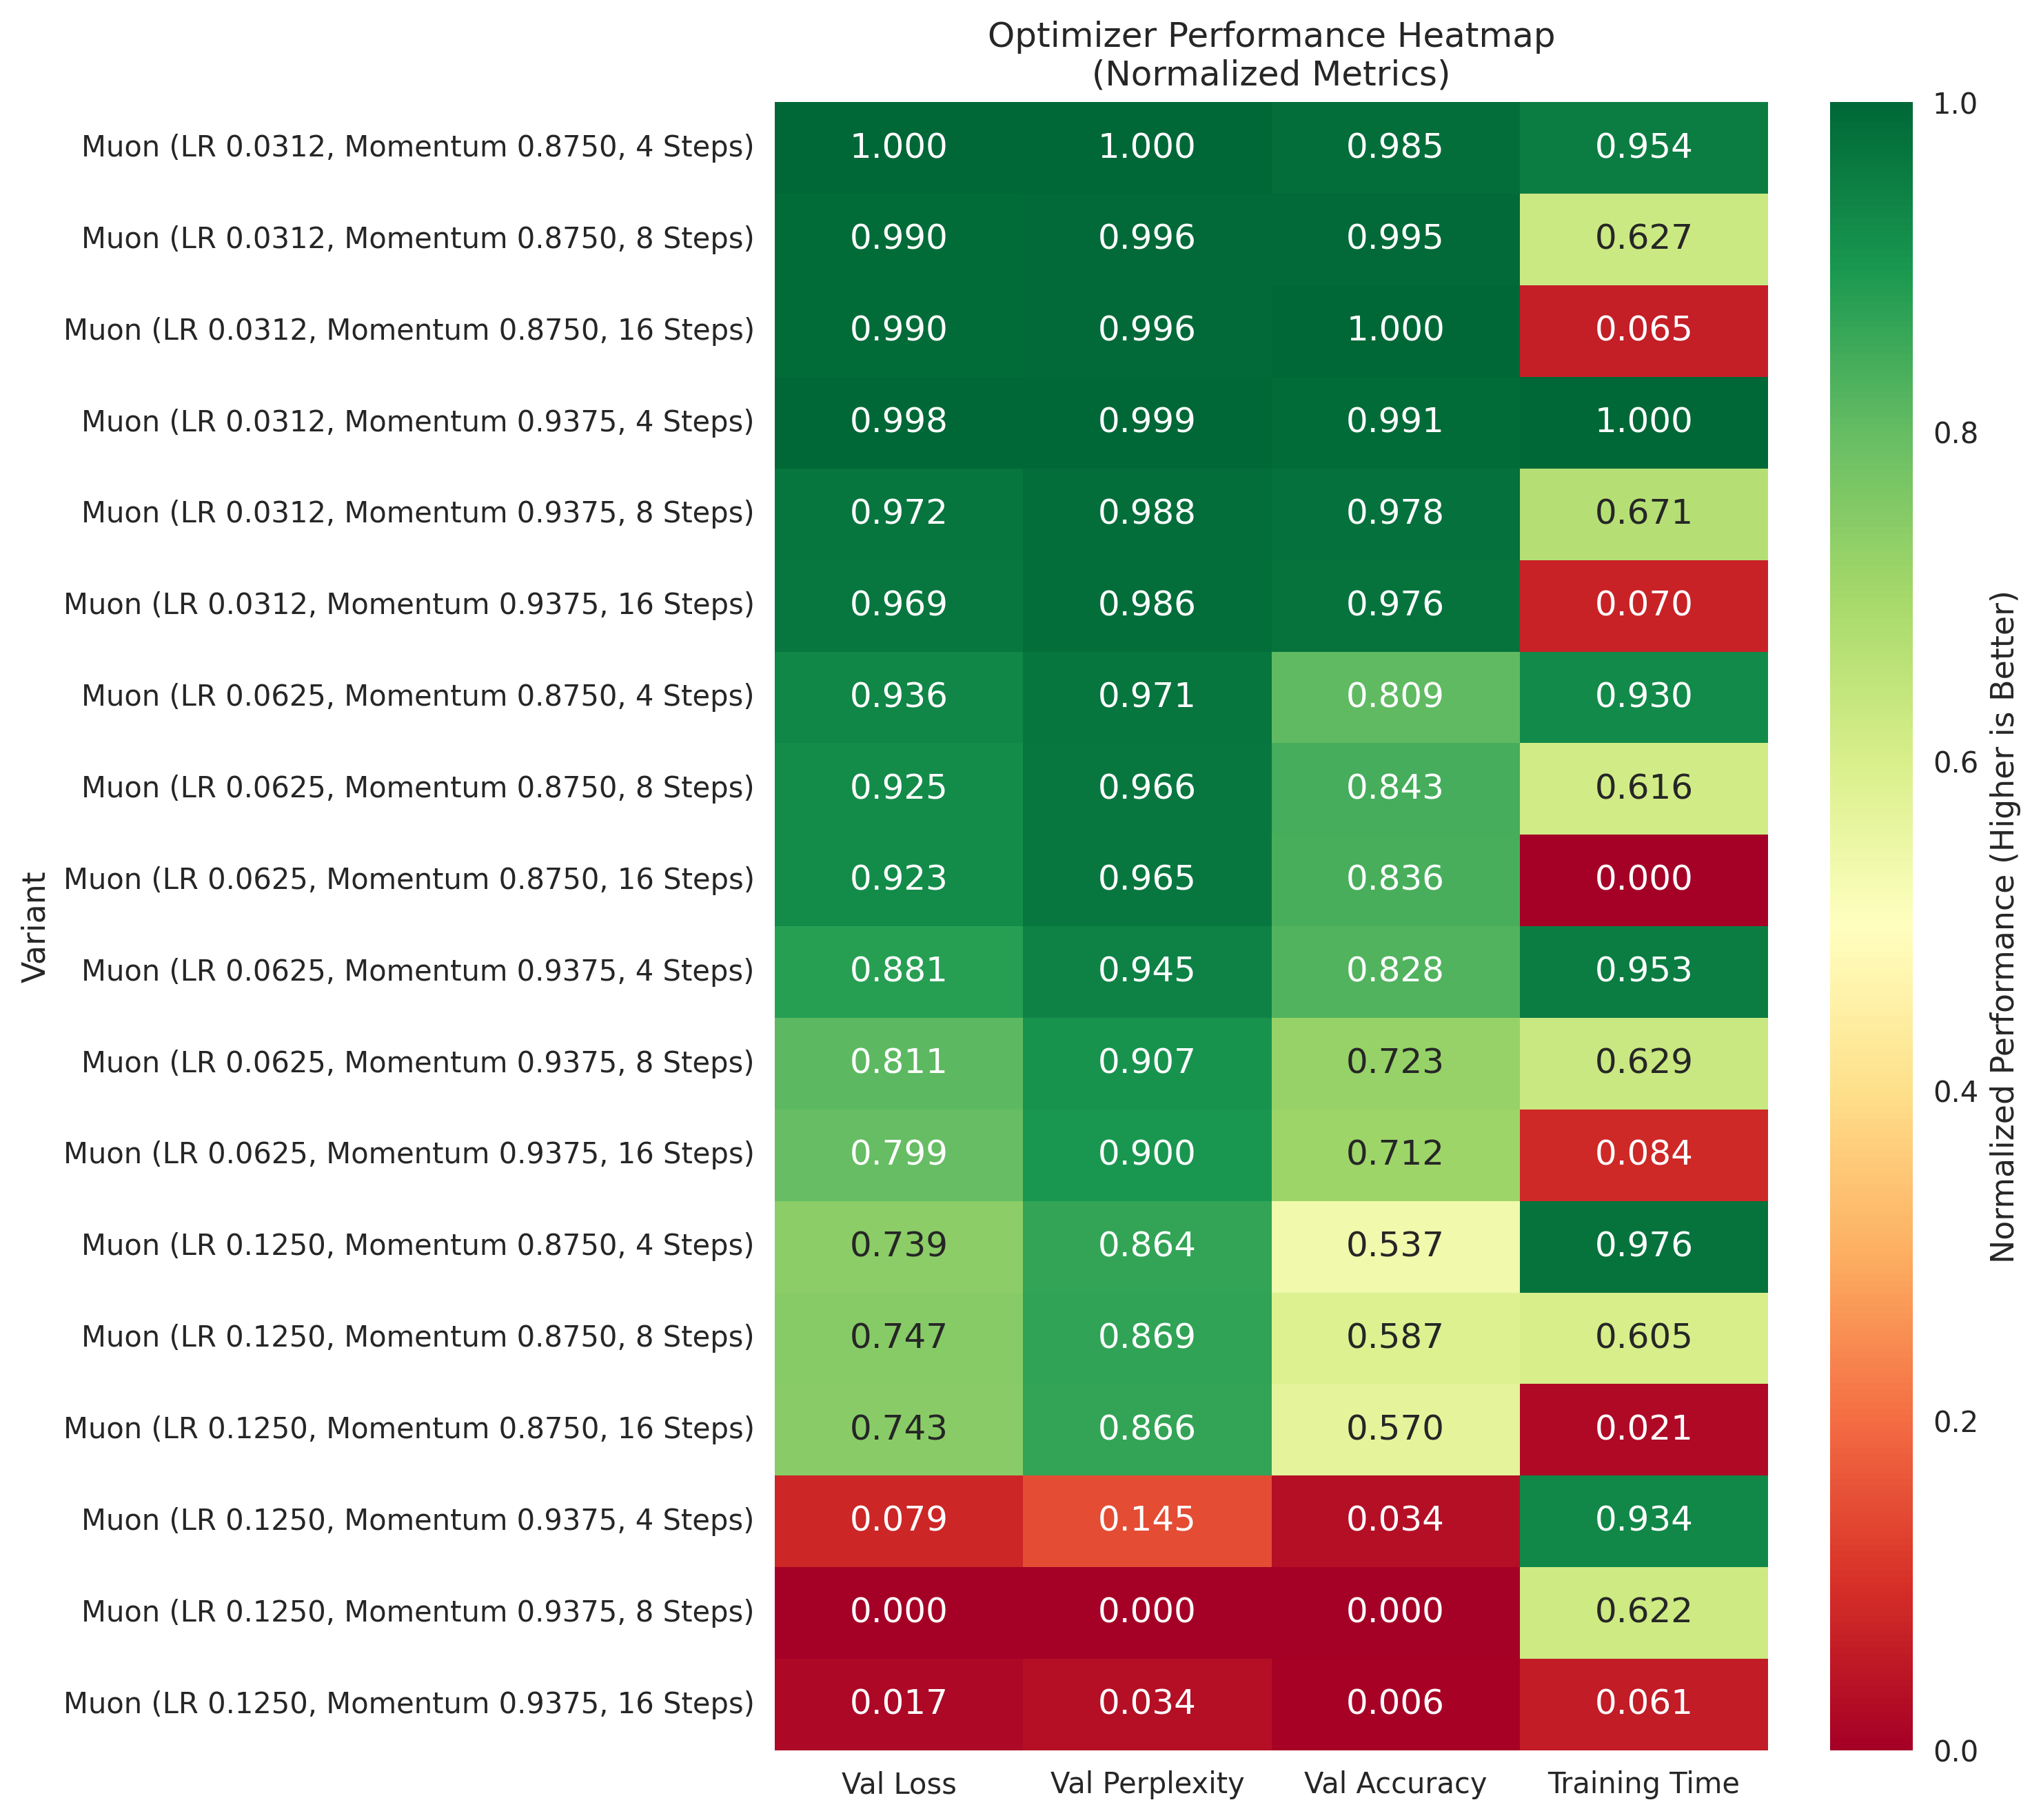
\includegraphics[width=\linewidth]{images/performance_heatmap.png}
    \caption{Performance heatmap showing normalized metrics across all configurations. Green indicates superior performance, red indicates poor performance. The heatmap clearly shows the dominance of low learning rate configurations.}
    \label{fig:heatmap_analysis}
\end{figure}

\subsection{Momentum and Newton-Schulz Steps Analysis}
Within learning rate groups, secondary effects emerge:

\textbf{Momentum Effects:}
\begin{itemize}
    \item At LR 0.0312: Momentum 0.8750 slightly outperforms 0.9375 (4 of 6 best configs)
    \item At LR 0.0625: Momentum 0.8750 consistently superior across all step counts
    \item At LR 0.1250: Momentum 0.8750 essential for stability (0.9375 leads to poor convergence)
\end{itemize}

\textbf{Newton-Schulz Steps Effects:}
\begin{itemize}
    \item Minimal impact on final performance within learning rate groups
    \item 4 steps achieve optimal balance of performance and computational efficiency
    \item 16 steps increase training time by 20\% with negligible performance gains
\end{itemize}

\subsection{Computational Efficiency Analysis}
Training times show predictable scaling with Newton-Schulz iterations:

\begin{table}[H]
\centering
\caption{Training Time Analysis by Newton-Schulz Steps}
\label{tab:timing_analysis}
\begin{tabular}{@{}lccc@{}}
\toprule
\textbf{Newton-Schulz Steps} & \textbf{Avg Time (s)} & \textbf{Time Overhead} & \textbf{Performance Impact} \\
\midrule
4 Steps & 131.4 & Baseline & Optimal for most configs \\
8 Steps & 140.7 & +7.1\% & Marginal performance change \\
16 Steps & 157.0 & +19.5\% & No consistent improvement \\
\bottomrule
\end{tabular}
\end{table}

\section{Discussion}

\subsection{Key Findings and Practical Implications}

\textbf{Learning Rate Criticality:} Our results demonstrate that learning rate selection is paramount for Muon optimizer performance. The clear performance tiers suggest that practitioners should prioritize conservative learning rate choices (≤0.03125) when computational budget allows for longer training.

\textbf{Momentum Stability:} Lower momentum values (0.8750) provide more consistent performance across learning rate settings, particularly important for high learning rate regimes where stability becomes critical.

\textbf{Newton-Schulz Efficiency:} The minimal performance difference between 4, 8, and 16 Newton-Schulz steps suggests that 4 iterations provide the optimal computational efficiency trade-off, reducing training time by 19.5\% compared to 16 steps with equivalent performance.

\textbf{Optimization Landscape:} The dramatic performance degradation at LR 0.1250 with momentum 0.9375 (ranks 16-18) indicates potential instability in the Muon optimizer's Newton-Schulz iterations under aggressive optimization settings.

\subsection{Recommendations for Practitioners}

Based on our systematic evaluation, we recommend:

\begin{enumerate}
    \item \textbf{Primary Configuration:} Start with LR 0.0312, momentum 0.8750, 4 Newton-Schulz steps
    \item \textbf{Resource-Constrained Scenarios:} LR 0.0312, momentum 0.9375, 4 steps (fastest training at 130s)
    \item \textbf{Stability-Critical Applications:} Avoid LR > 0.0625 with momentum > 0.8750
    \item \textbf{Computational Optimization:} Use 4 Newton-Schulz steps unless specific precision requirements demand higher iteration counts
\end{enumerate}

\subsection{Limitations and Future Work}

\subsection{Limitations and Future Work}

\textbf{Model Scale Limitations:} Our study employs a deliberately small model architecture (128-dimensional, 2 layers) to enable comprehensive hyperparameter exploration within computational constraints. While this approach allows systematic analysis, the findings may not directly generalize to production-scale language models with billions of parameters. Future work should investigate hyperparameter sensitivity in larger model regimes.

\textbf{Training Duration Constraints:} The 1500-step training duration, while sufficient for comparative analysis, represents a fraction of typical language model training schedules. Extended training runs (10K+ steps) may reveal different hyperparameter dynamics, particularly regarding learning rate scheduling and momentum adaptation over longer optimization trajectories.

\textbf{Hardware Limitations:} Experiments were conducted on a single NVIDIA RTX 3070 GPU with 8GB VRAM, limiting model size and batch size exploration. Future studies with high-memory GPUs or distributed training setups could explore larger model configurations and investigate hyperparameter scaling behavior.

\textbf{Dataset Scope:} Results are based on the cosmopedia-v2 subset of smollm-corpus, representing a specific text domain. Different text types (code, scientific literature, conversational data) may exhibit varying sensitivity to Muon optimizer hyperparameters, warranting domain-specific optimization studies.

\textbf{Optimizer Comparison:} Our study focuses exclusively on Muon optimizer variants without systematic comparison to established optimizers (AdamW, SGD, Lion). Future work should provide comprehensive optimizer benchmarking to contextualize Muon's relative performance advantages.

\textbf{Future Research Directions:}
\begin{itemize}
    \item Investigation of hyperparameter scaling laws for larger model architectures
    \item Dynamic hyperparameter adaptation strategies during extended training
    \item Cross-domain validation across diverse NLP tasks and text types
    \item Integration with learning rate scheduling and warmup strategies
    \item Memory-efficient implementations for larger-scale deployment
    \item Theoretical analysis of Newton-Schulz iteration convergence properties
\end{itemize}

\section{Conclusion}

This comprehensive ablation study provides empirical guidance for Muon optimizer hyperparameter selection in language modeling applications. Our systematic evaluation of 18 configurations reveals that learning rate selection is the dominant factor affecting performance, with optimal results achieved at conservative learning rates (0.0312) combined with moderate momentum (0.8750) and minimal Newton-Schulz iterations (4 steps).

The study demonstrates that effective optimization with Muon requires careful hyperparameter tuning, particularly for learning rate selection, where aggressive settings can lead to substantial performance degradation. For practitioners implementing Muon optimization, our results suggest prioritizing stability over aggressive optimization, with the recommended configuration achieving validation loss of 4.3998 while maintaining computational efficiency.

These findings contribute to the growing body of knowledge on second-order optimization methods and provide a foundation for future research into adaptive optimization strategies for transformer-based language models.

\section*{References}

\begin{thebibliography}{9}

\bibitem{jordan2024muon}
Keller Jordan, Yuchen Jin, Vlado Boza, Jiacheng You, Franz Cesista, Laker Newhouse, and Jeremy Bernstein.
\newblock Muon: An optimizer for hidden layers in neural networks.
\newblock 2024.
\newblock \url{https://kellerjordan.github.io/posts/muon/}

\bibitem{kingma2014adam}
Diederik P. Kingma and Jimmy Ba.
\newblock Adam: A method for stochastic optimization.
\newblock \textit{arXiv preprint arXiv:1412.6980}, 2014.

\bibitem{loshchilov2017decoupled}
Ilya Loshchilov and Frank Hutter.
\newblock Decoupled weight decay regularization.
\newblock In \textit{International Conference on Learning Representations}, 2019.

\bibitem{vaswani2017attention}
Ashish Vaswani, Noam Shazeer, Niki Parmar, Jakob Uszkoreit, Llion Jones, Aidan N Gomez, Łukasz Kaiser, and Illia Polosukhin.
\newblock Attention is all you need.
\newblock \textit{Advances in neural information processing systems}, 30, 2017.

\bibitem{chen2023symbolic}
Xiangning Chen, Chen Liang, Da Huang, Esteban Real, Kaiyuan Wang, Yao Liu, Hieu Pham, Xuanyi Dong, Thang Luong, Cho-Jui Hsieh, Yifeng Lu, and Quoc V. Le.
\newblock Symbolic discovery of optimization algorithms.
\newblock \textit{arXiv preprint arXiv:2302.06675}, 2023.

\bibitem{martens2020new}
James Martens, Jimmy Ba, and Matt Johnson.
\newblock Kronecker-factored approximate curvature for modern neural network architectures.
\newblock In \textit{Advances in Neural Information Processing Systems}, 33, 2020.

\end{thebibliography}

\end{document}